\documentclass[10pt]{article}
\usepackage{amsmath} 
\usepackage{fontspec}
\usepackage[a4paper, margin=12mm]{geometry}
\usepackage{graphicx}
\usepackage{titlesec}
\usepackage{amsmath}
\usepackage{fancyhdr}
\usepackage{amsmath}
\usepackage{datetime}
\usepackage[hidelinks]{hyperref}
\usepackage[utf8]{inputenc}
\usepackage{booktabs}

\setmainfont{JetBrains Mono}
\setmainfont[NFSSFamily=dayrom]{JetBrains Mono}
\graphicspath{ {./images/} }

\DeclareSymbolFont{digits}{TU}{dayrom}{m}{n}
\AtBeginDocument{
	\DeclareMathSymbol{0}{\mathalpha}{digits}{`0}
	\DeclareMathSymbol{1}{\mathalpha}{digits}{`1}
	\DeclareMathSymbol{2}{\mathalpha}{digits}{`2}
	\DeclareMathSymbol{3}{\mathalpha}{digits}{`3}
	\DeclareMathSymbol{4}{\mathalpha}{digits}{`4}
	\DeclareMathSymbol{5}{\mathalpha}{digits}{`5}
	\DeclareMathSymbol{6}{\mathalpha}{digits}{`6}
	\DeclareMathSymbol{7}{\mathalpha}{digits}{`7}
	\DeclareMathSymbol{8}{\mathalpha}{digits}{`8}
	\DeclareMathSymbol{9}{\mathalpha}{digits}{`9}
}

% subsubsubsection
\titleclass{\subsubsubsection}{straight}[\subsection]
\newcounter{subsubsubsection}[subsubsection]
\renewcommand\thesubsubsubsection{\thesubsubsection.\arabic{subsubsubsection}}
\renewcommand\theparagraph{\thesubsubsubsection.\arabic{paragraph}} % optional; useful if paragraphs are to be numbered

\titleformat{\subsubsubsection}
{\normalfont\normalsize\bfseries}{\thesubsubsubsection}{1em}{}
\titlespacing*{\subsubsubsection}
{0pt}{3.25ex plus 1ex minus .2ex}{1.5ex plus .2ex}

\makeatletter
\renewcommand\paragraph{\@startsection{paragraph}{5}{\z@}%
	{3.25ex \@plus1ex \@minus.2ex}%
	{-1em}%
	{\normalfont\normalsize\bfseries}}
\renewcommand\subparagraph{\@startsection{subparagraph}{6}{\parindent}%
	{3.25ex \@plus1ex \@minus .2ex}%
	{-1em}%
	{\normalfont\normalsize\bfseries}}
\def\toclevel@subsubsubsection{4}
\def\toclevel@paragraph{5}
%\def\toclevel@paragraph{6}
\def\toclevel@subparagraph{6}
\def\l@subsubsubsection{\@dottedtocline{4}{7em}{4.5em}}
\def\l@paragraph{\@dottedtocline{5}{10em}{5em}}
\def\l@subparagraph{\@dottedtocline{6}{14em}{6em}}
\makeatother

\setcounter{secnumdepth}{4}
\setcounter{tocdepth}{4}


\hypersetup{
	colorlinks=true,
	urlcolor=cyan,
}

% Footer-Einstellungen
\newdateformat{mydate}{\twodigit{\THEDAY}.\twodigit{\THEMONTH}.\THEYEAR}
\mydate
\pagestyle{fancy}
\fancyhf{} % Löscht alle Kopf- und Fusszeilen
\fancyfoot[C]{\thepage\ -\ \today\ \copyright\ Bastian\ Kind,\ James\ Binks,\ Mark\ Matkovic\ und\ David\ Hafner} % Setzt den Footer
\begin{document}
	\section{Band C}
	\subsection{Elemente einer Benutzerschnittstelle kennen und anwenden}
	\subsubsection{Controls und Widgets erklären}
	\subsubsubsection{Was sind controls und Widgets}
	Controls oder Widgets sind grafische Steuerelemente einer Benutzeroberfläche. Sie ermöglichen dem Benutzer, mit einem Programm zu interagieren, Eingaben zu machen und Informationen zu erhalten. Controls und Widgets sind nicht alle Interaktionselemente, da mache nur für die datenübergabe an den Nutzer sind.
	
	\subsubsubsection{Häufig verwendete Controls und Widgets}
	\begin{tabular}{@{}lll@{}}
		\toprule
		\textbf{Widget / Control} & \textbf{Beschreibung} & \textbf{Wichtige Eigenschaften} \\
		\midrule
		Button (Schaltfläche) & Ein klickbares Element, das eine Aktion auslöst. & Text, Icon, aktiv/deaktiviert \\
		Label (Beschriftung) & Zeigt Text oder Information an, keine Interaktion. & Text, Schriftart, Ausrichtung \\
		Textfeld (Textbox) & Ermöglicht die Eingabe von Text durch den Benutzer. & Inhalt, Länge, Passwortmodus, aktiv/deaktiviert \\
		Checkbox (Kontrollkästchen) & Ermöglicht das An- oder Abwählen einer Option. & An/Aus-Zustand \\
		Radiobutton (Optionsfeld) & Ermöglicht das Auswählen einer Option aus einer Gruppe. & Gruppenzugehörigkeit, Auswahlstatus \\
		Dropdown (Auswahlliste) & Ermöglicht die Auswahl eines Werts aus einer Liste. & Ausgewählter Wert, Listeneinträge \\
		Slider (Schieberegler) & Ermöglicht das Einstellen eines Werts innerhalb eines Bereichs. & Minimalwert, Maximalwert, aktueller Wert \\
		Progressbar (Fortschrittsanzeige) & Zeigt den Fortschritt eines Vorgangs an. & Minimalwert, Maximalwert, aktueller Wert \\
		Image (Bild) & Zeigt ein Bild oder Icon an. & Dateipfad, Größe, Skalierung \\
		\bottomrule
	\end{tabular}
	
	\subsubsection{Controls und Widgets sinvoll verwenden}
	\subsubsubsection{was bedeutet sinvoll plaziert}
	Sinvoll plazierte Widgets und Controlls sorgen dafür das der Nutzer die Seite möglichst Intuitive und Effizient navigieren kann. Unteranderem sollten einfach erkenbare Symbole verwendet werden und diese sollte an den gewohnten stellen plaziert sein. Wenn ein User nach etwas sucht, dann sollte er ohne lange suchen zu müssen fündig werden.\\
	Wir haben unsere Symbole und die Plazierung der Element, vor allem in der Nav bar, von der SRF Webseite inspirieren lassen, da diese Seite stark besucht ist und damit unsere Applikation unseren Usern schon bekannt vor kommen sollte.
	\\
	\subsubsubsection{Sinvolle Umsetzung}
	In userer Umsetzung haben wir die ERlernte Theorie angewendet. Die Navbar und die Suchfunktion ist wie bei SRF und sollte den meisten Kunden bereits bekannt vorkommen.
	\\
	Der Hauptinhalt der Seite ist die Interaktive Karte.
	\\
	Unsere Footer Bar besteht aus 3 gängigen Symbolen.
	\begin{itemize}
		\item QR-Code
		\item Map
		\item Einstellungszahnrad
	\end{itemize}
	Das sind alles sehr gängige Symbole welche für fast jeden sofort verständlich sein sollten.\\\\
	Unsere Search funktion ist auch auf SRF basiert und ist so Intuitive wie möglich gestalltet. Alle möglichen Aktionen sind sofort Zentral ersichtlich. Der hintergrund wird aus dem Fokus genommen damit die neuen Interaktionsmöglichkeiten herausstechen und die zuvor besuchte Seite immer noch so halb ersichtlich ist, dies sollte sicherstellen das die Nutzer wissen das die vorherige Seite nicht verloren gegangen ist.\\\\
	Die Settingspage ist bekannten überkategorien organisiert mit der Accessibility ganz oben damit man schnell den Screenreader oder die Schriftgrösse zu seinen präferenzen ändern kann.<
	\\
	\subsubsection{Controls und Widgets in eine Logische abfolge bringen}
	Durch Umfgragen mit mehreren Dritten personen und Inspirationen von verschiedenen Webseiten haben wir die Plazierung und die Zusammenareit unserer Controlls und Widgets Optimiert. Wir haben unseren Fokus auch auf einen Logischen Aufbau gelegt damit es für jeden, auch für Kinder oder Ältere personen, einfach verstehen können. Unsere Applikation ist jetzt sehr intuitive und sollte für jeden brauchbar sein.
	\\
	
	\subsection{Benutzerschnittstelle erstellen und testen}
	\subsubsection{Skitzen als Prototyp umsetzen}
	Ich habe micht dazu entschieden, den Prototypen als Webseite zu bauen. Bei der Arbeit entwickle ich auch Webseiten. Deshalb geht das für mich einfacher, als ein neues Tool zu lernen. Wenn wir dann die richtige App programmieren würden, könnten wir auch den Code aus dem Prototypen weiter verwenden.\\
	Hier ist der Link zur \href{https://davidhafner.github.io/M322-Documentation/}{Webseite}\\\\
	
	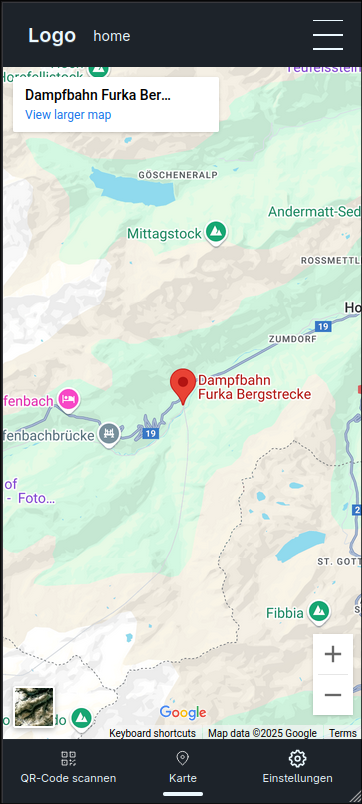
\includegraphics[width=7cm ]{mainpage}
	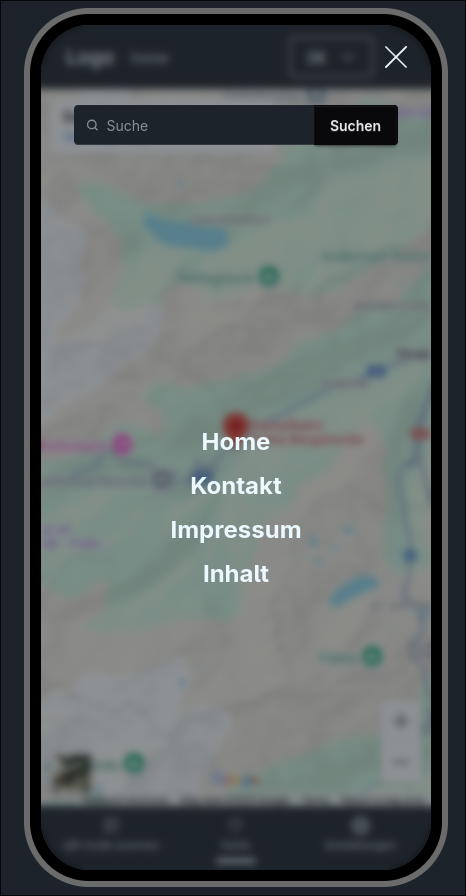
\includegraphics[width=7cm ]{searchpage}
	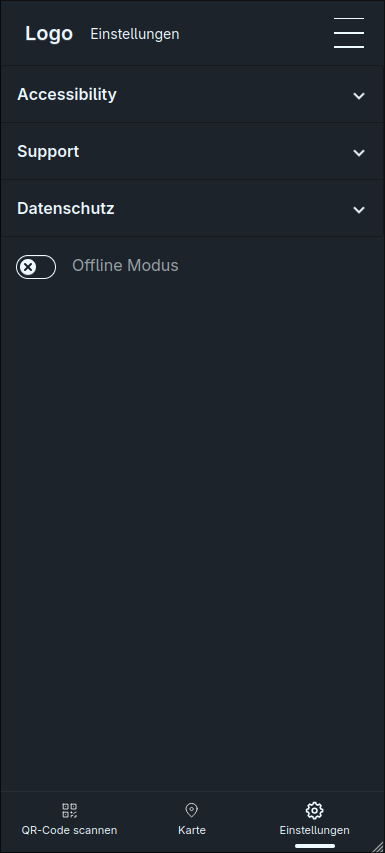
\includegraphics[width=7cm]{settingspage}
	\\\\
	\subsubsection{Testen und Probleme indentifizieren}
	\begin{itemize}
		\item Den Prototypen habe ich nur für die Mobile ansicht optimiert. Im Desktopmodus sieht er nicht so gut aus.
		\item Wenn man mit dem Menu von einer Seite zu einer anderen wechselt bleibt das Menu offen. Das ist nicht intuitiv.
		\item Da ich im Browser den Dark mode verwende, sieht sie im light mode nicht so gut aus.
	\end{itemize}
	\subsubsection{Verbesserungen}
	\begin{itemize}
		\item Da der Prototyp nur für Mobile optimiert sein muss, könnte ich es auf grossen Bildschirmen in ein Handy packen. So kann man die Webseite trotzdem gut testen.
		\item Wenn im Menu eine Seite gewählt wird, werde ich machen, dass das Menu automatisch schliesst.
		\item Ich werde die Webseite im light mode testen.
	\end{itemize}
	

	
	
	\subsection{Benutzerfreundlichkeit verbessern}
	

	
\end{document}